\documentclass[12pt]{article}
\setlength{\oddsidemargin}{0in}
\setlength{\evensidemargin}{0in}
\setlength{\textwidth}{6.5in}
\setlength{\parindent}{0in}
\setlength{\parskip}{\baselineskip}
\usepackage{amsmath,amsfonts,amssymb}
\usepackage{graphicx}
\usepackage{float}
\usepackage{enumitem}
\usepackage[]{algorithmicx}
\usepackage{amsthm}
\usepackage{fancyhdr}
\pagestyle{fancy}
\setlength{\headsep}{36pt}
\usepackage{tkz-berge}
\usetikzlibrary{positioning, automata}

\theoremstyle{remark}
\newtheorem*{solution}{Solution}

\usepackage{listings}% http://ctan.org/pkg/listings
\lstset{
  basicstyle=\ttfamily,
  mathescape
}

\usepackage{hyperref}



\newcommand{\makenonemptybox}[2]{%
%\par\nobreak\vspace{\ht\strutbox}\noindent
\item[]
\fbox{% added -2\fboxrule to specified width to avoid overfull hboxes
% and removed the -2\fboxsep from height specification (image not updated)
% because in MWE 2cm is should be height of contents excluding sep and frame
\parbox[c][#1][t]{\dimexpr\linewidth-2\fboxsep-2\fboxrule}{
  \hrule width \hsize height 0pt
  #2
 }%
}%
\par\vspace{\ht\strutbox}
}
\makeatother

\begin{document}
\definecolor {processblue}{cmyk}{0.96,0,0,0}
\lhead{{\bf CSCI 3104, Algorithms \\ Final Exam - 100 pts total} }
\rhead{Name: Luna McBride \\ ID: 107607144 \\ {\bf Profs.\ Hoenigman \& Agrawal\\ Fall 2019, CU-Boulder}}
\renewcommand{\headrulewidth}{0.5pt}

\phantom{Test}
\noindent
{\bf Notes:}
%\noindent
\begin{itemize}
\item {\em Due date: 6pm on Sunday, December 8, 2019}
\vspace{-2mm}
\item {\em Submit a pdf file of your written answers to Gradescope and one py file with your Python codes to Canvas. All Python solutions should be clearly commented. Your codes need to run to get credit for your answers.}
\vspace{-2mm}
\item {\em You can ask clarification questions about the exam in office hours and on Piazza. However, please do not ask questions about how to answer a specific question. If there is confusion about any questions, we will address those issues at the beginning of class on December 5.}
\vspace{-2mm}
\item {\em All work on this exam needs to be independent. You may consult the textbook, the lecture notes and homework sets, but you should not use any other resources. If we suspect that you collaborated with anyone in the class or on the Internet, we will enforce the honor code policy strictly. If there is a reasonable doubt about an honor code violation,  you will fail this course.}
\end{itemize}
%\vspace{2mm}

\hrulefill

\begin{enumerate}
\item (10 pts) Consider the following merge() algorithm to merge two sorted arrays into a larger sorted array. There are three errors in the algorithm. 
\begin{verbatim}
MergeWithErrors(A, p, q, r)
    low = A[p..q]
    high = A[q..r]
    i = 0
    j = 0
    k = p
    while(i < q-p+1 and j < r-q)
        if(low[i] <= high[j])
            A[k] = low[i]
            j++
        else
            A[k] = high[j]
            i++
        k++
    while(i < q-p+1)
        A[k] = low[i]
        i++
        k++
    while(j < r-q)
        A[k] = high[j]
        j++
        k++
\end{verbatim}
\begin{enumerate}
    \item (5 pts) List the three errors in the MergeWithErrors algorithm.
    \begin{solution}
    $\newline$ 1) high is A[q..r] when it should be A[q+1..r], otherwise the q would overlap. $\newline$ 2) in the "if(low[i] $<$= high[j])" statement, the j++ should be i++, as it is coresponding to the low array and not the high. $\newline$ 3) in the else of the previous statement, the i++ should be j++ for the reason before, just with low and high swapped.
    \end{solution}
    \pagebreak
    
    \item (5 pts) For the following call to MergeWithErrors, what is the state of the array $A$ after running MergeWithErrors. You can assume that the size of $A$ won't change and values written outside the indices of $A$ will be lost.
    \\ $$A=[0,1,3,5,2,4,6,7]$$
     $$MergeWithErrors(A, 0, 3, 7)$$
    \begin{solution}
    $\newline$$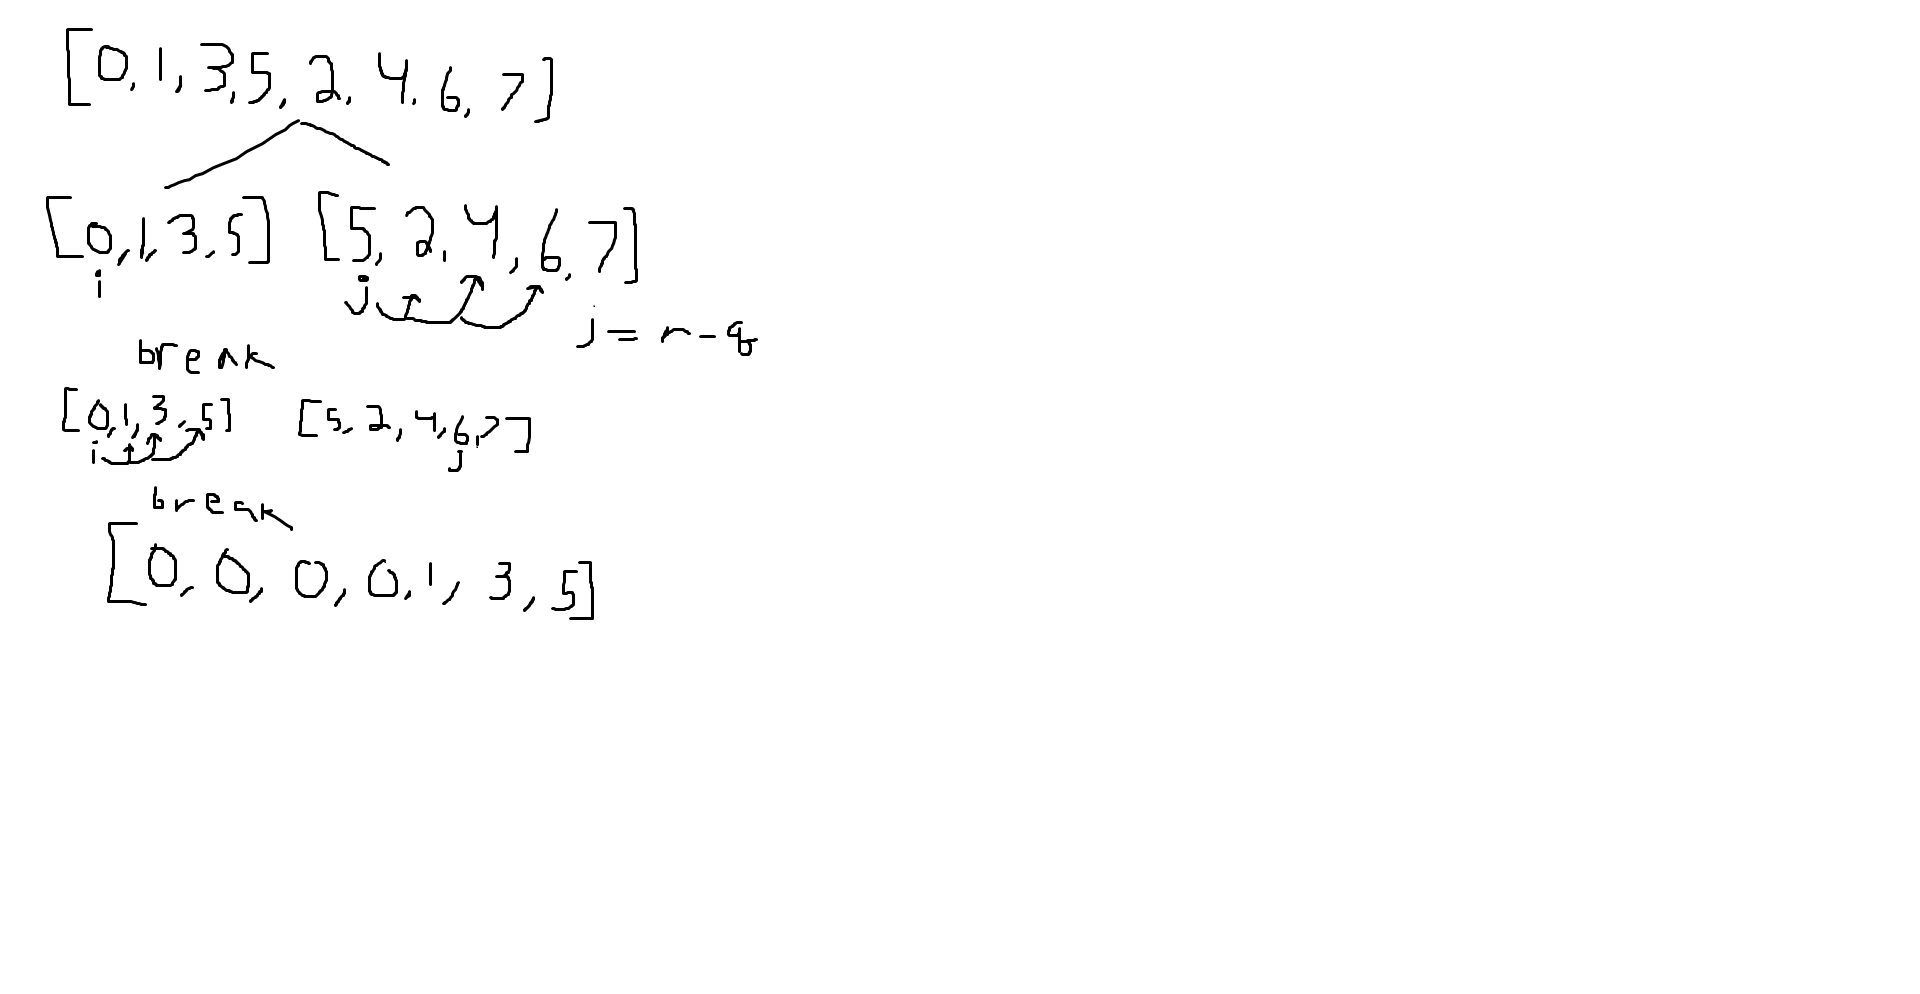
\includegraphics[scale=0.5]{bad}$$\newline$
    \end{solution}
    \pagebreak
    
\end{enumerate}


\item (25 pts) Let $G=(V,E)$ be a directed weighted graph of the pathways on the CU-Boulder campus, with edge weights being distances between different buildings/intersections. Engineering and Humanities are two vertices of $G$, and $k>0$ is a given integer. Assume that you will stop at every building/intersection you pass by. A shortest $k$-stop path is a shortest path between two vertices with exactly $k$ stops.
\begin{enumerate}
    \item (5 pts) Provide an example showing that the shortest $k$-stop path can't necessarily be found using Breadth-first search or Dijkstras algorithm. You need an example for each algorithm that shows where it fails.
    \begin{solution}
    $\newline$ $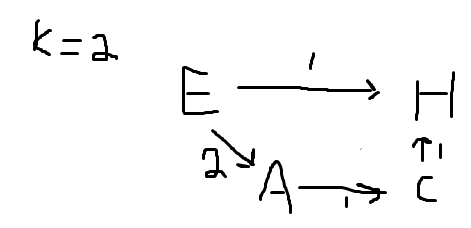
\includegraphics[scale=0.5]{dijbad}$$\newline$ In this example, Dijkstra's algorithm will not follow the rules and go directly to H, which, sure is less, but it is non-stop and not the required 2
$\newline$ $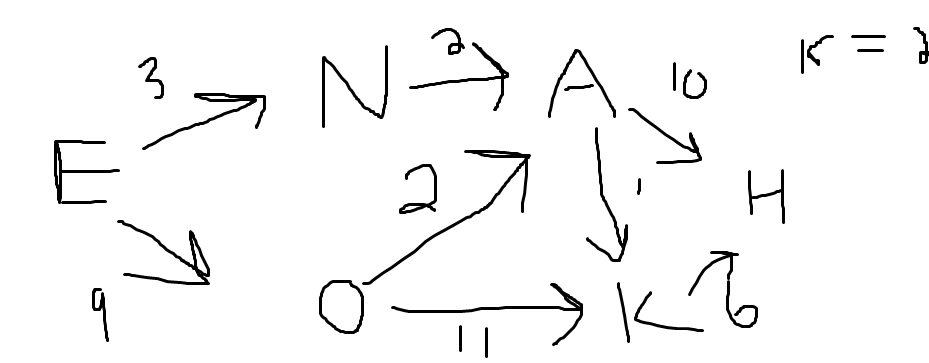
\includegraphics[scale=0.5]{bfsbad}$$\newline$ With Breadth First, it more tells how many hops it needs instead of going through each for its weights. This means in this crazy mess, while it is easy for it to get to the k, it is unlikely to find the most optimal by weight
    \end{solution}
    \pagebreak

    \item (10 pts) Design an algorithm to find the shortest path from Engineering to Humanities that contains exactly $k$ stops (excluding Engineering and Humanities). Notice that a $k$-stop path from these two buildings may not exist. So, your algorithm should also take care of such possibility. You need to provide an explanation of how your algorithm works to receive credit for this question.
    \begin{solution}
\begin{verbatim}
    def path(G):
    g=[[("EC",0,None)]]
    k=7
    c=0
    e=0
    while c==0:
        for i in range(0,len(g[e])):
            #for j in range(0,len(g[e][i])):
            q=[]
            w=g[e][i][0]
            p=list(G[w])
            for l in range(0,len(p)):
                if p!=None:
                    q.append((p[l],g[e][i][1]+float(G[w][p[l]]["weight"]),g[e][i][0]))
            g.append(q)
        if e==k:
            c=1
        print(g[e],'\n\n')
        e+=1

    e=e-1
    ww=[]
    print(g[k])
    for n in range(0,len(g[k])):
        if g[k][n][0]=='HUMN':
            ww.append(g[k][n])

    if len(ww)==0:
        return []
    else:
        c=99
        r=0
        for j in range(0,len(ww)):
            c=min(c,ww[j][1])
            r=j

    return ww[j]
\end{verbatim}
$\newline$ Please note this is not complete. I have run out of time and need to get to work. However, I hope you can see the ideas I was trying to put in place working with the q2 starter code. This starts with the given k (actually representing k-1 because we are seeing if it is humanities). This does a breadth first approach to go about getting to the given k. It then sees if there are any humanities in the list at this k (that is k+1). The initial plan was to go through and implement a call back function after finding the humn with the least weight, but I ran out of time to fully work on with no late period allowed, so I tried my best (saved 2 for last)
    \end{solution}
    \pagebreak

    \item (10 pts) Implement your algorithm using the starter code provided on Canvas. 
    
\end{enumerate}

\item (25 pts) To entertain her kids during a recent snowstorm, Dr. Hoenigman invented a card game called EPIC!. In the two-player game, an even number of cards are laid out in a row, face up so that players can see the cards' values. On each card is written a positive integer, and players take turns removing a card from either end of the row and placing the card in their pile. The objective of the game is to collect the fewest points possible. The player whose cards add up to the lowest number after all cards have been selected wins the game.
\\One strategy is to use a greedy approach and simply pick the card at the end that is the smallest. However, this is not always optimal, as the following example shows: (The first player would win if she would first pick the 5 instead of the 4.)

4 2 6 5

\begin{enumerate}
\item (10 pts) Write a non-greedy, efficient and optimal algorithm for a strategy to play EPIC!. The runtime needs to be less than $\theta(n^2)$. Player 1 will use this strategy and Player 2 will use a greedy strategy of choosing the smallest card. \textbf{Note: Your choice of algorithmic strategy really matters here. Think about the types of algorithms we've learned this semester when making your choice.} You need to provide an explanation of how your algorithm works to receive credit for this question.
$\pagebreak$
    \begin{solution} $\newline$
    def epic(A,p,r):  $\newline -->$
    if p==r: $\newline --/-->$
        return A[p] $\newline -->$
    if r-p==1: $\newline --/-->$
        return min(A[p],A[r]) $\newline -->$
    if (A[p]+A[r-1])$>$(A[r]+A[p+1]) and A[p]$>$A[r]: $\newline --/-->$
        return A[r] $\newline -->$
    if (A[p]+A[r-1])$<$(A[r]+A[p+1]) and A[p]$<$A[r]: $\newline --/-->$
        return A[p] $\newline -->$
    if (A[p]+A[r-1])$<$(A[r]+A[p+1]): $\newline --/-->$
        return A[p] $\newline -->$
    return A[r]  $\newline \newline$ This function is specifically used for a single turn. This specifically uses the thought process of the importance of looking one ahead specifically, using p as the current left side and r as the current right. it looks one ahead and compares like I would do when doing a turn like this with my human brain. The turn emulator will then go through this and greedy switching off to emulate players, which is not shown here because this is to emulate a single turn for player 1. $\newline \newline$ Interestingly, I do not believe there is a way to work this game without having even the optimal win 100 percent of the time, specifically because of cases like this one, when the optimal is player 1: [ 8  4  9 10  3  6  2  7  1  5].
    \end{solution}
    \pagebreak

\item (15 pts) Implement your strategy and the greedy strategy in Python and include code to simulate a game. Your simulation work for up to 100 cards, and values ranging from 1 to 100. Your simulation should include a randomly generated collection of cards and show the sum of cards in each hand at the end of the game. 
\end{enumerate}

\pagebreak
\item (22 pts) 
	In a previous homework assignment and classroom activity, we worked on the problem of finding the peak in an array, where array $A[1, 2, \cdots, n]$ with the property that the subarray $A[1..i]$ has the property that $A[j]>A[j+1]$ for $1\leq j< i$, and the subarray $A[i..n]$ has the property that $A[j]<A[j+1]$ for $i\leq j < n$. For example, $A=[16, 15, 10, 9, 7, 3, 6, 8, 17, 23]$ is a peaked array.\\
	
	Now consider the \textit{multi-peaked} generalization, in which the array contains $k$ peaks, i.e., it contains $k$ subarrays, each of which is itself a peaked array. Suppose that $k=2$ and we can guarantee that neither peak is closer than $n/4$ positions to the middle of the array, and that the ``joining point'' of the two singly-peaked subarrays lays in the middle half of the array. 
	\begin{enumerate}
	    \item (8 pts) Now write an algorithm that returns the minimum element of $A$ in sublinear time.
	    \begin{solution}
    $\newline$ def mini(A,p,r): $\newline -->$  q=floor($\frac{p+r}{2}$)  $\newline -->$ if r-p+1==3: $\newline --/-->$ return A[q] $\newline -->$ if A[q] $>$ A[q-1] and A[q]$<$A[q+1]:  $\newline --/-->$ min(mini(A,p,q), mini(A,q,r))  $\newline -->$ elif A[q]$>$A[q+1] and A[q]$<$A[q-1]:  $\newline --/-->$ return A[q]  $\newline -->$ elif A[q]$>$A[q+1]:  $\newline --/-->$ return mini(A,q,r)  $\newline -->$ else:  $\newline --/-->$ return mini(A,p,q)
        \end{solution}
        \pagebreak

	    \item (10 pts) Prove that your algorithm is correct. (Hint:\ prove that your algorithm's correctness follows from the correctness of another correct algorithm we already know.)
	    \begin{solution}
    $\newline$ Base Case: the array only has 3 elements, peak in the middle as to fit the definition of a peaked array. k=1, so the min is just the peak, A[middle]. $\newline \newline$ Inductive Hypothesis: The relation holds for k peaks. $\newline \newline$ Inductive Step: Case 1: A[middle] is a joining point. Call each side and take its minimum, as to get the minimum of the peaks in each section, which are the minimum parts of the peaked section. $\newline$ Case 2: A[middle] is the peak. return that, which is called as the peak following a single-peak algorithm just appended to the other little mountains, which is either taken as the minimum overall or returned as the call to be compared to previous k peaks. $\newline$ Case 3: A[middle] is on the slope on an upward incline (it is greater than the next value). This returns a call that will return the peak when it comes upon it later. The call is to values q...r (middle...r), which holds either a section to the end of the peak on a single peak or potentially multiple peaks depending on the size, which will keep becoming smaller by further calls. $\newline$ Case 4: A[middle] is on a downward decline, meaning there is at least one peak before it. The previous values in the array are then called in hopes to find a peak, which will be called until it is small enough to count for one peak while being compared to others as it starts coming back up

        \end{solution}
        \pagebreak

	    \item (4 pts) Give a recurrence relation for its running time, and solve for its asymptotic behavior.
	   \begin{solution}
    $\newline$ T(n)=T(n/2)+$n^0$ $\newline \newline$ $log_2{1}$?0 $\newline$ 0=0 $\newline$ O(log(n))
        \end{solution}
        \pagebreak

	\end{enumerate}

\item (18 pts) Suppose we are given a set of non-negative distinct numbers $S$ and a target $t$. We want to find if there exists a subset of $S$ that sums up to \textbf{exactly} $t$ and the cardinality of this subset is $k$. 
\\Write a python program that takes an input array $S$, target $t$, and cardinality $k$, and returns the subset with cardinality $k$ that adds to $t$ if it exists, and returns $False$ otherwise. Your algorithm needs to run in $O(ntk)$ time where $t$ is the target and $n$ is the cardinality of $S$. In your code, provide a brief discussion of your runtime through comments, referring to specific elements of your code.\\
\\For example - 

Input: s = \{2,1,5,7\}, t = 4, k = 2\\
Output: False\\
Explanation:  No subset of size $2$ sums to 4.\\\\
Input: s = \{2,1,5,7\}, t = 6, k = 2\\
Output: \{1, 5\}\\
Explanation:  Subset \{1, 5\} has size 2 and sums up to the target $t = 6$.\\\\
Input: s = \{2,1,5,7\}, t = 6, k = 3\\
Output: False\\
Explanation:  No subset of size $3$ sums to 6.\\\\

\noindent
\end{enumerate}





\end{document}

